\chapter{Diseño e Implementación}


\section{Modelado de la base de datos}
En un primer diagrama para la base de datos se exponen las entidades y sus realciones. Atendiendo a los requisitos de la aplicación se plantea un diseño sencillo y directo en cuanto a las entidades y relaciones. En un primer esquema \textbf{entidad-relación} encontramos:



\begin{figure}[!ht]
  \begin{center}
    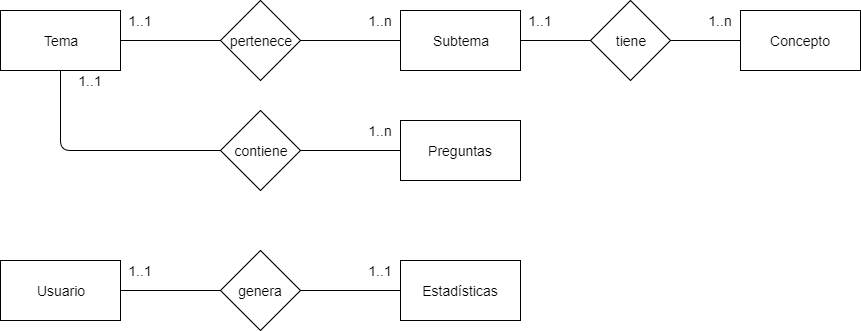
\includegraphics[width=1\textwidth]{../images/entidad_relacion.png}
    \caption{Entidad relación}
    \label{fig:entidad_relacion}
  \end{center}
\end{figure}


\bigskip
Analizando el diagrama vemos que las únicas relaciones que existen son de cardinalidad 1:N y 1:1.
Ambas las podemos simplificar eliminando la relación y añadiendo la clave primaria de la entidad con cardinalidad 1 en los campos de la entidad con cardinalidad N. Quedan así resumidas las tablas de la base de datos a únicamente las entidades:

\begin{figure}[!ht]
  \begin{center}
    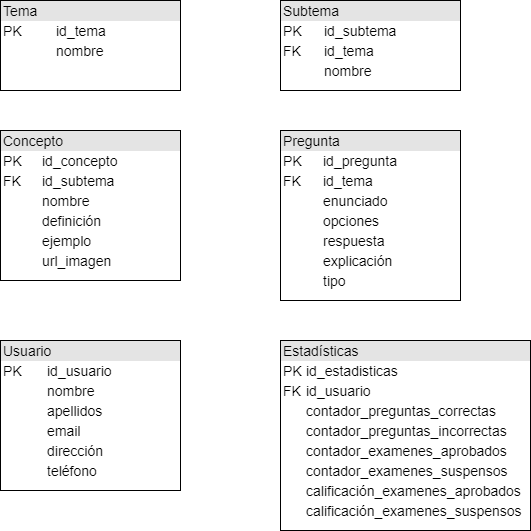
\includegraphics[width=1\textwidth]{../images/entidad_relacion_simplificado.png}
    \caption{Tablas del modelo entidad relación}
    \label{fig:entidad_relacion_simplificado}
  \end{center}
\end{figure}


\newpage

\section{Diseño de las interfaces}

A menudo y varias veces al día nos encontramos con cientos de interfaces\cite{user_exp2} con las que interactuamos, muchas de estas están tan asimiladas que ni las apreciamos. Las interfaces no son un objetivo para el usuario, si no que son el medio para llegar al él, siendo estas que no apreciamos las mejores interfaces. Una interfaz\cite{user_exp} no debe entorpecer el camino del usuario hasta su objetivo, debe ser sencilla, rápida de asimilar y directa.

\bigskip
Aquí mostramos algunos bocetos sencillos y su consiguiente implementación como interfaz de usuario en la aplicación:

\newpage

\subsection{Bocetos}

\begin{figure}[!ht]
  \begin{center}
    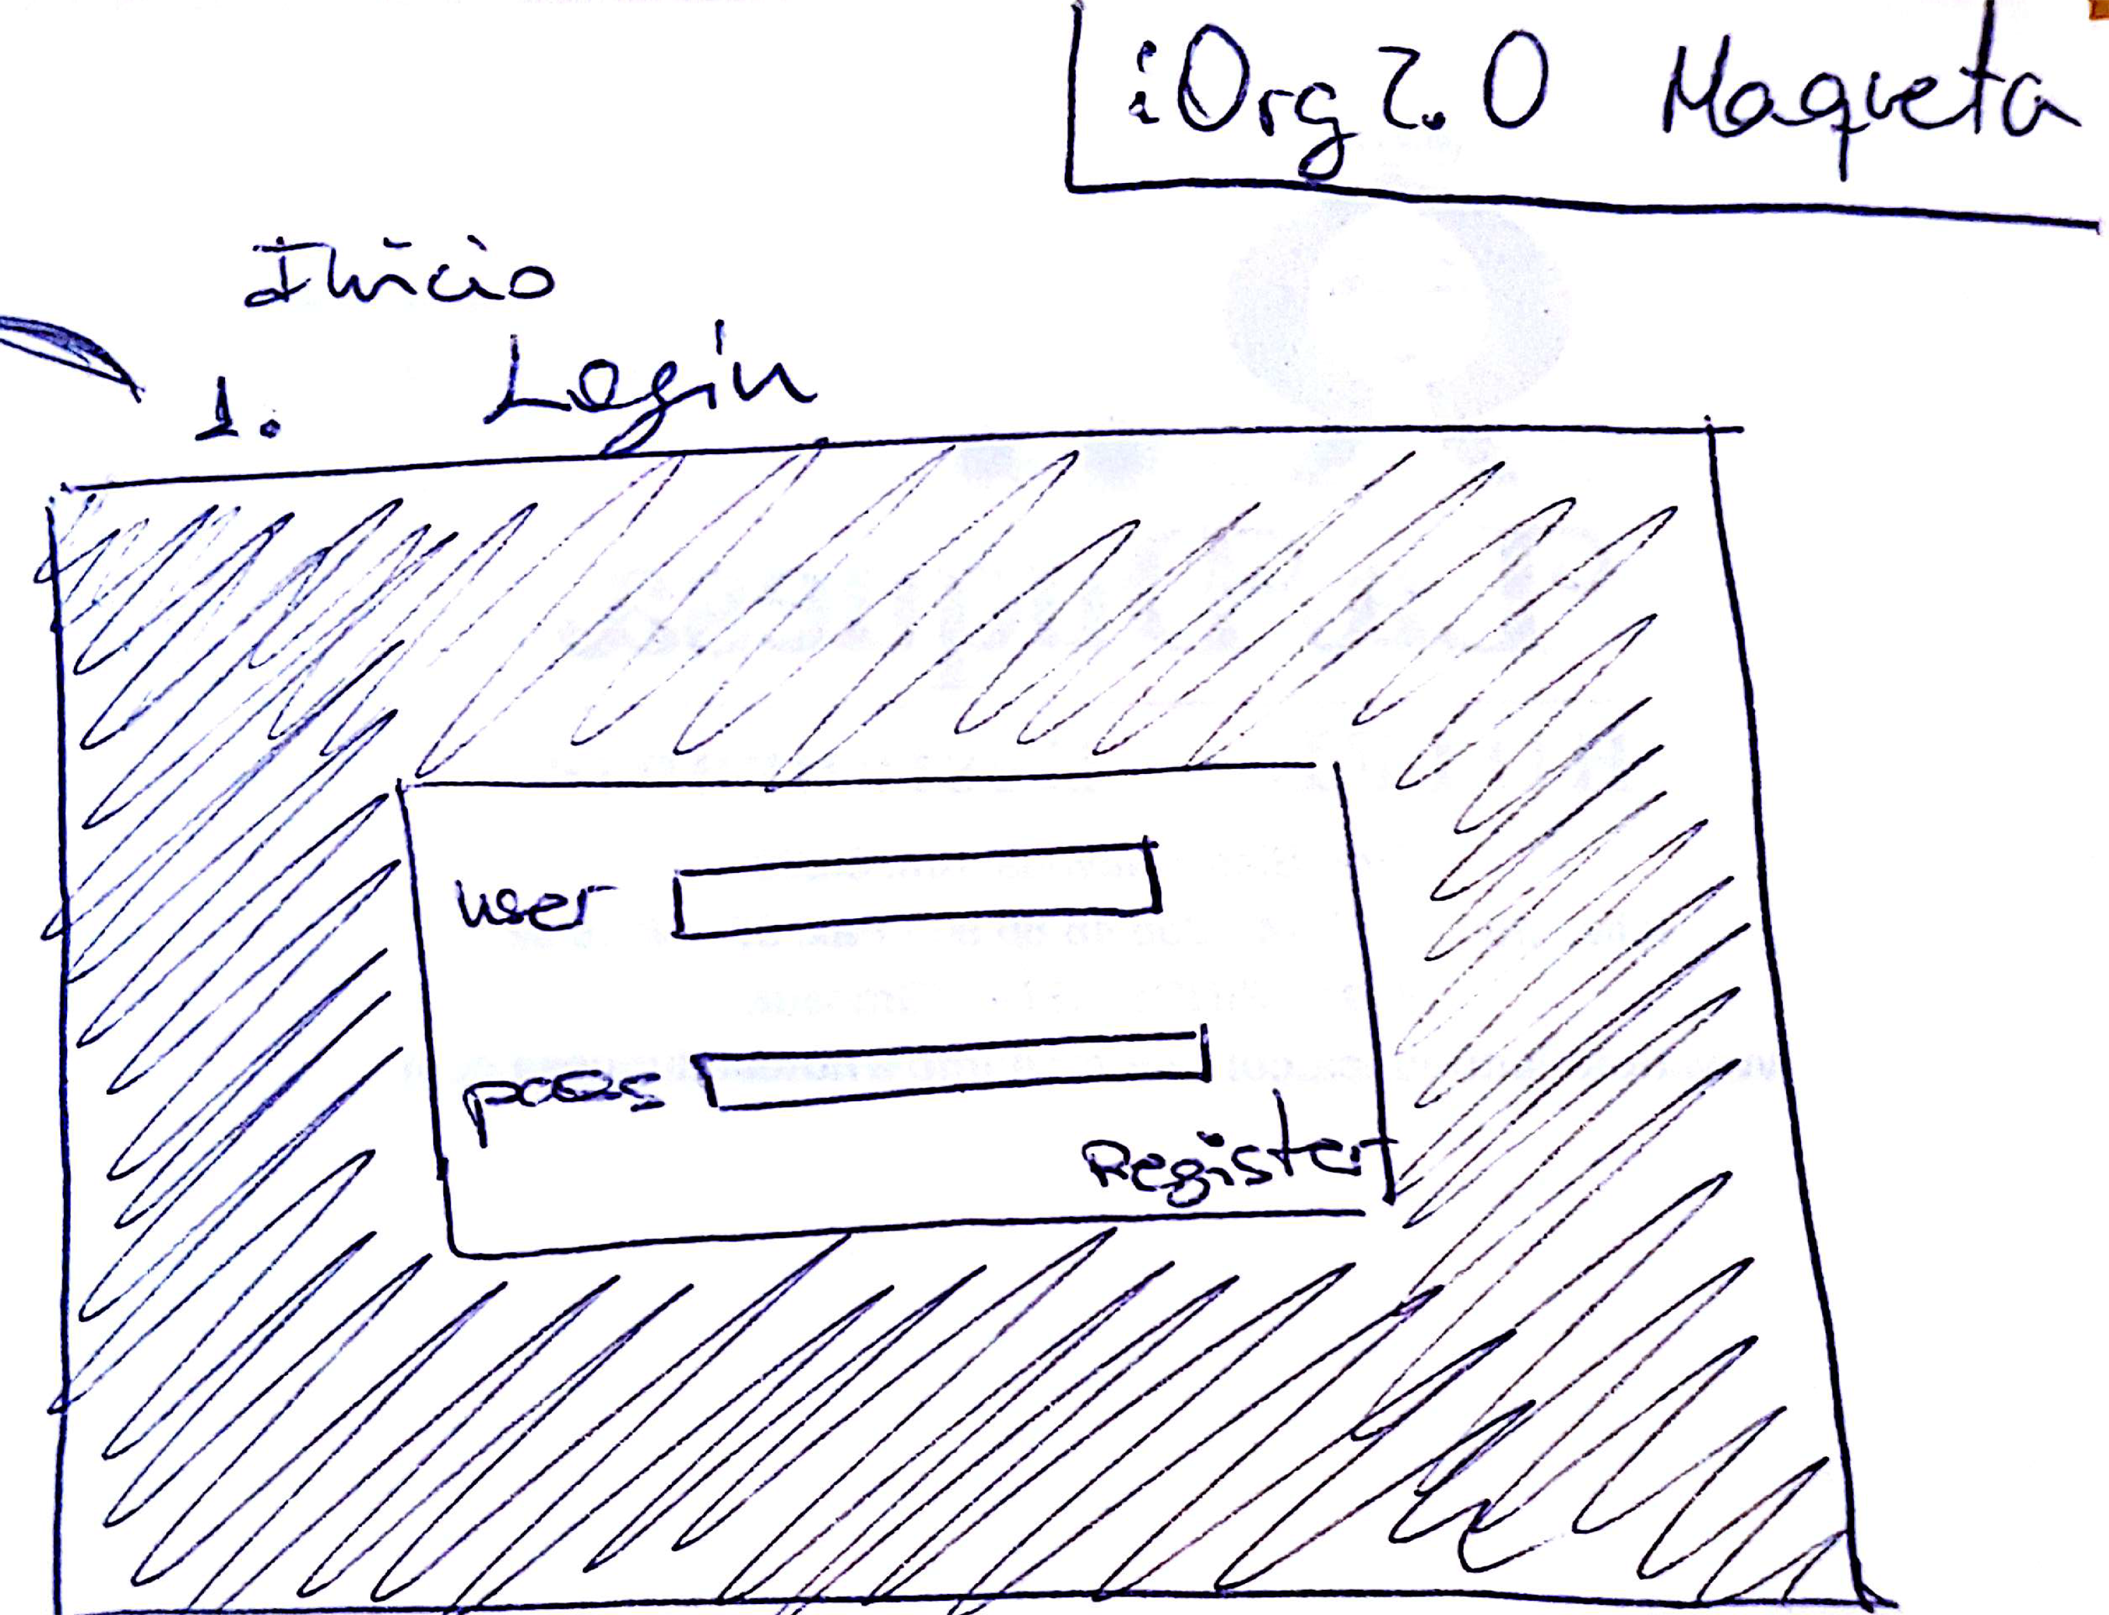
\includegraphics[width=1\textwidth]{../images/boceto_login.png}
    \caption{Boceto interfaz inicio de sesión.}
    \label{fig:boceto_login}
  \end{center}
\end{figure}


\begin{figure}[!ht]
  \begin{center}
    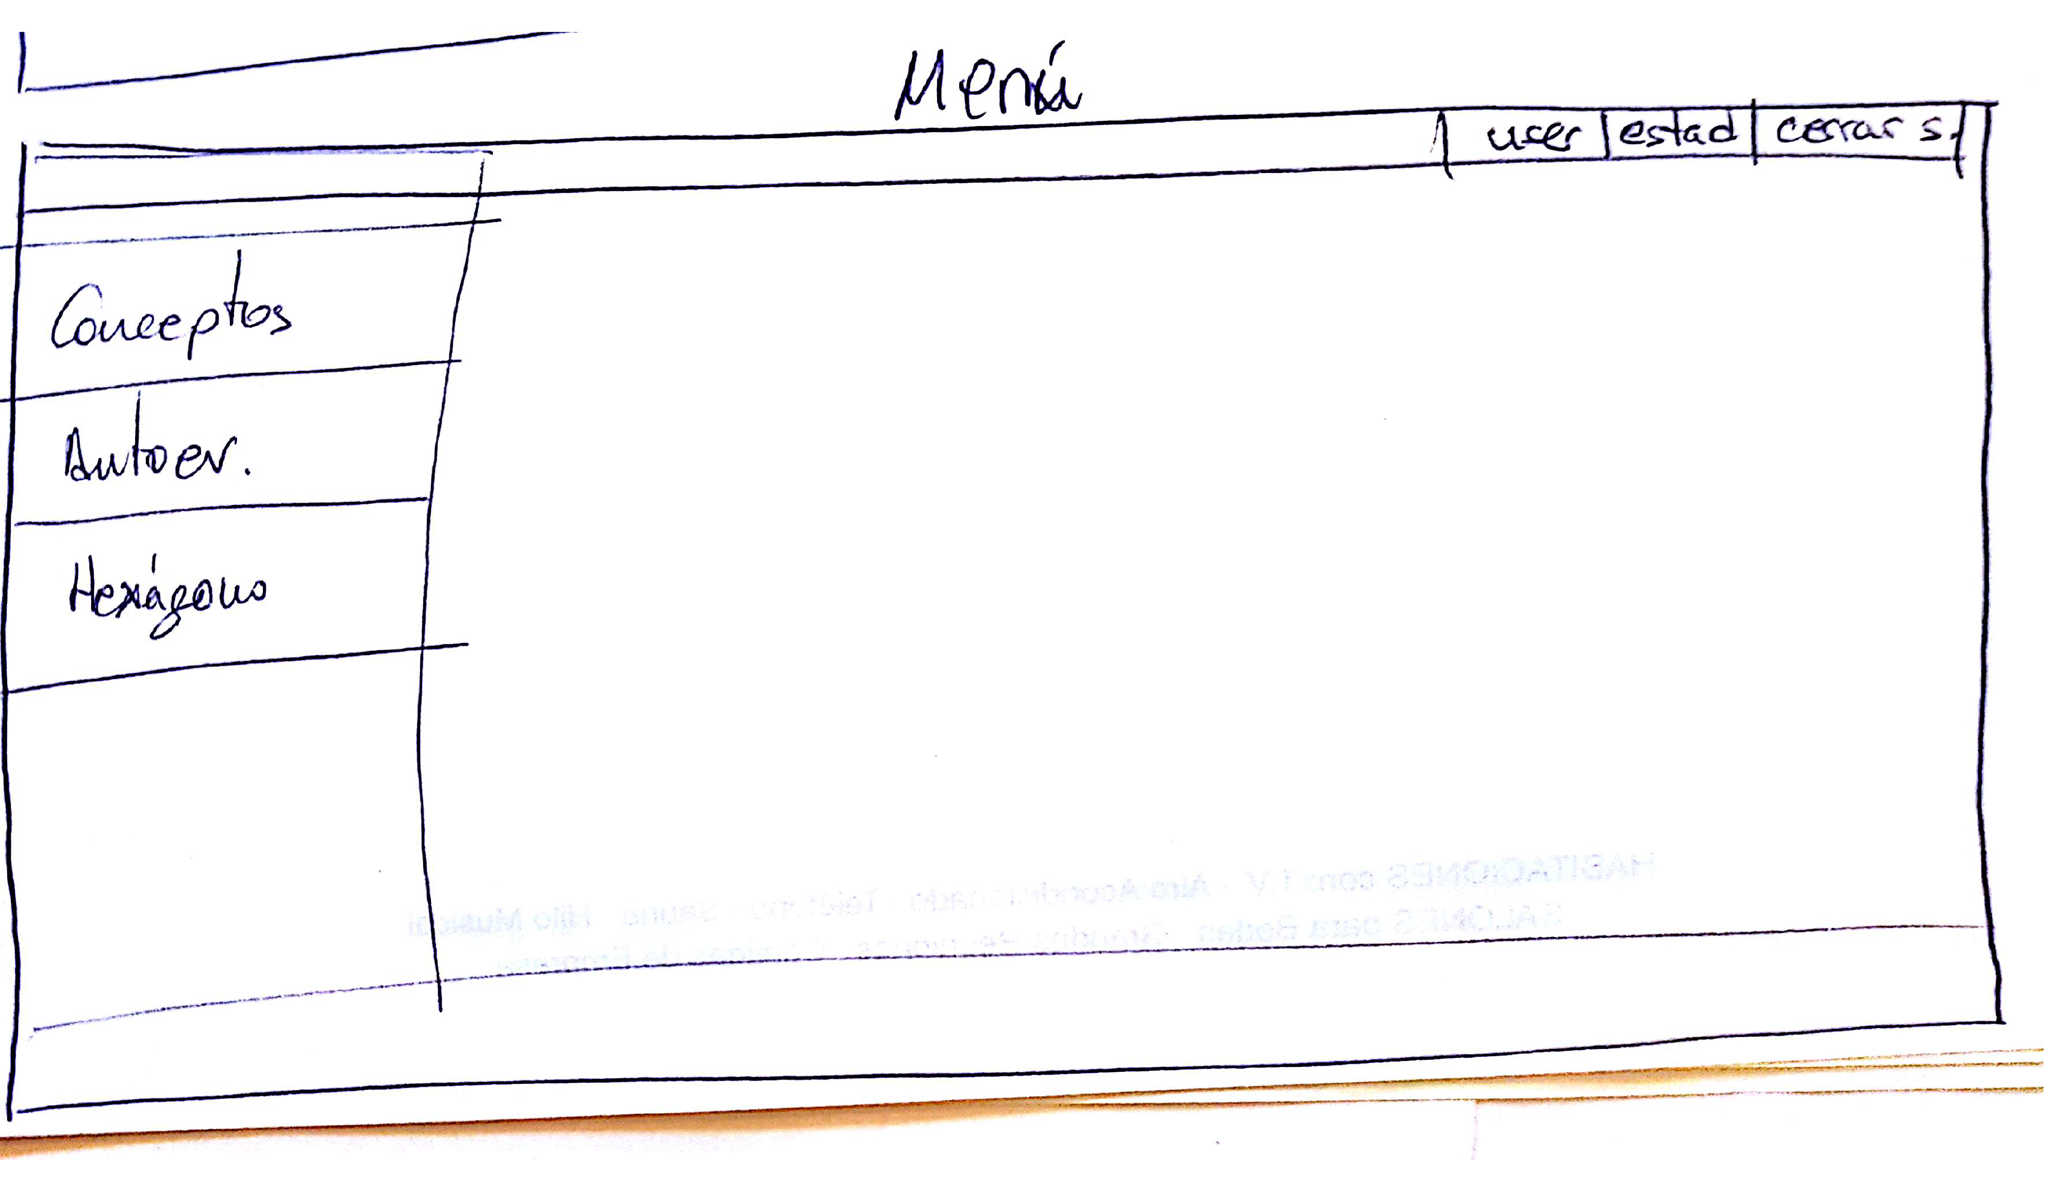
\includegraphics[width=1\textwidth]{../images/boceto_menu_lat.png}
    \caption{Boceto interfaz menú lateral.}
    \label{fig:boceto_menu_lat}
  \end{center}
\end{figure}



\begin{figure}[!ht]
  \begin{center}
    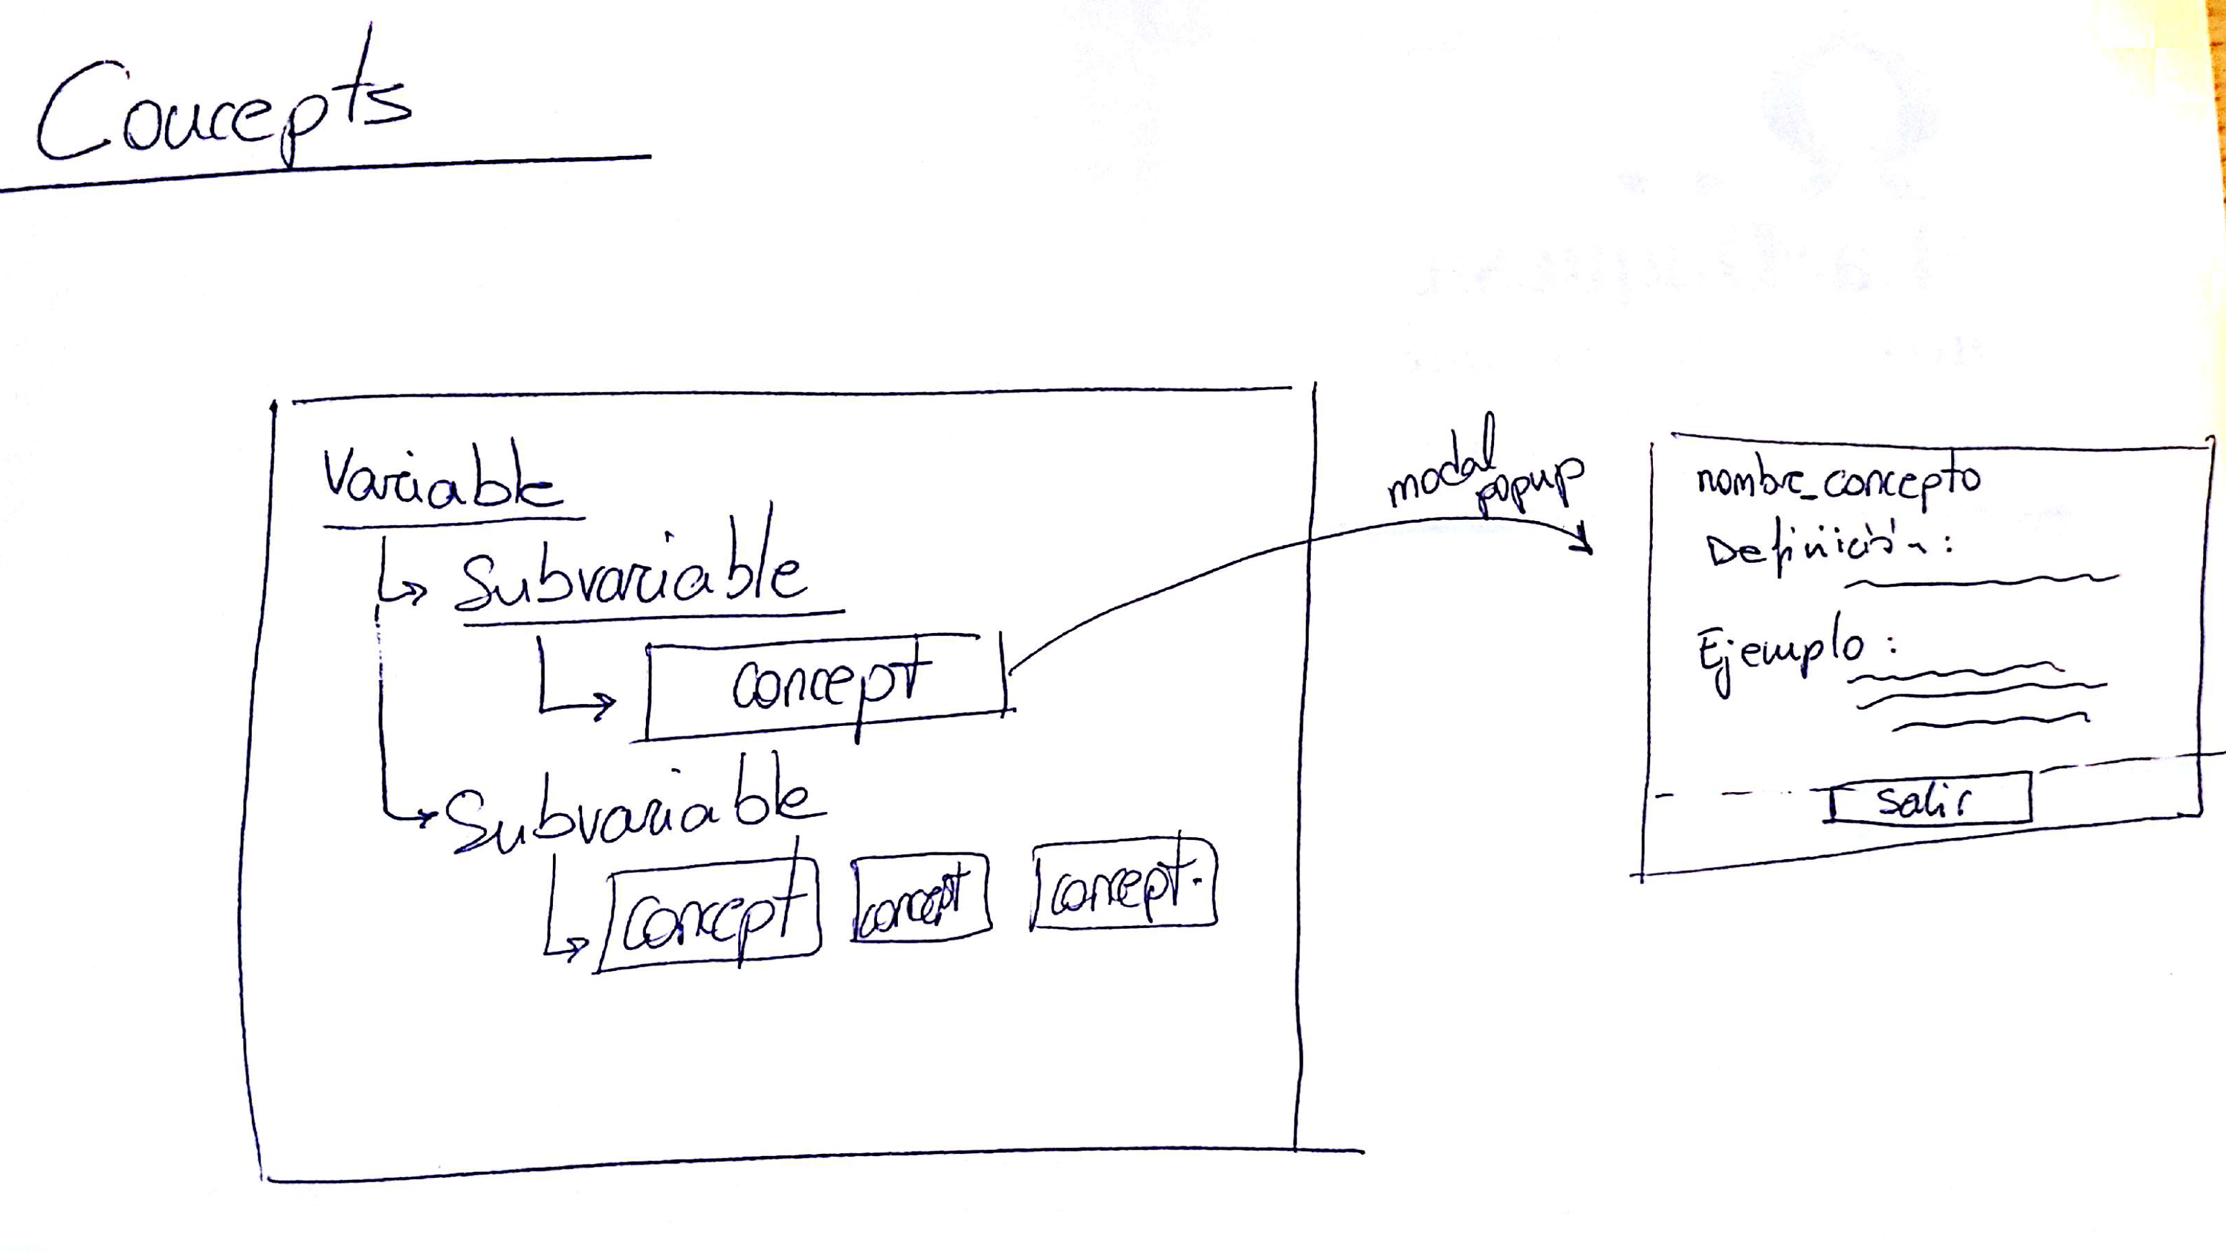
\includegraphics[width=1\textwidth]{../images/boceto_conceptos.png}
    \caption{Boceto interfaz conceptos.}
    \label{fig:boceto_conceptos}
  \end{center}
\end{figure}


\newpage

\subsection{Interfaz}

\begin{figure}[!ht]
  \begin{center}
    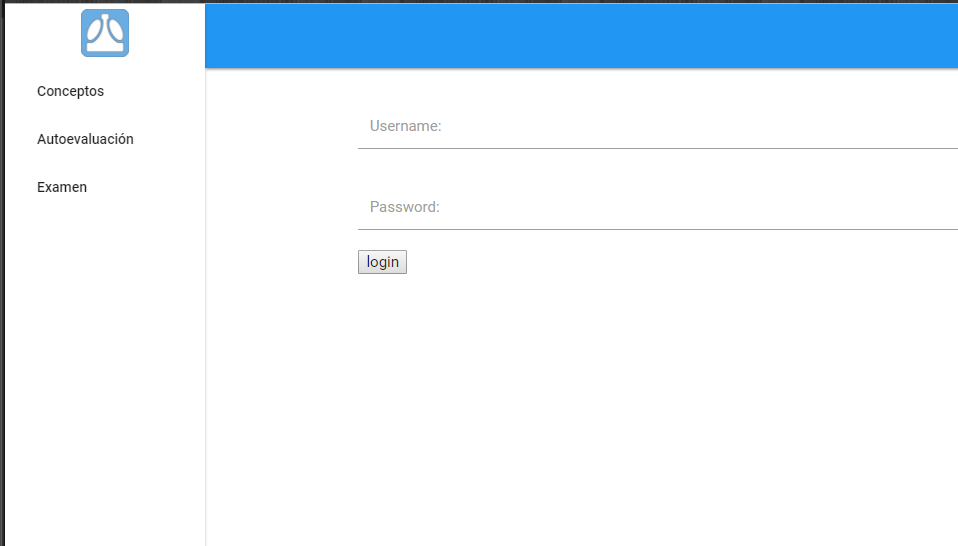
\includegraphics[width=1\textwidth]{../images/interfaz_login.png}
    \caption{Interfaz de usuario inicio de sesión.}
    \label{fig:interfaz_login}
  \end{center}
\end{figure}


\begin{figure}[!ht]
  \begin{center}
    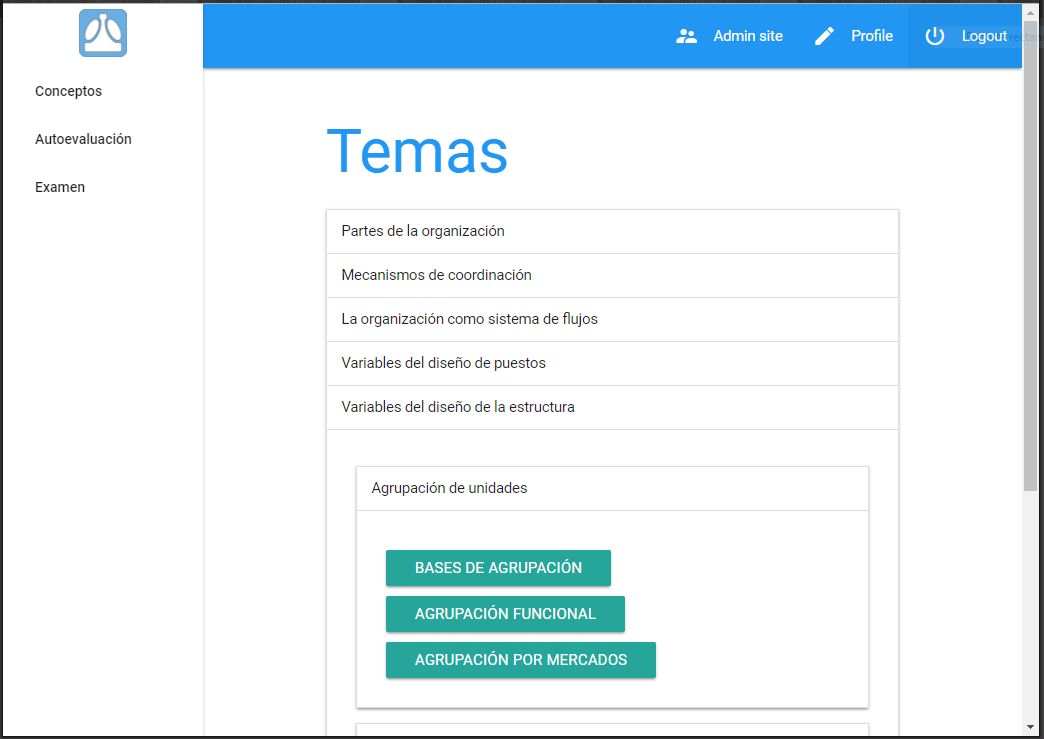
\includegraphics[width=1\textwidth]{../images/interfaz_conceptos1.png}
    \caption{Interfaz de usuario conceptos 1/2.}
    \label{fig:interfaz_conceptos1}
  \end{center}
\end{figure}



\begin{figure}[!ht]
  \begin{center}
    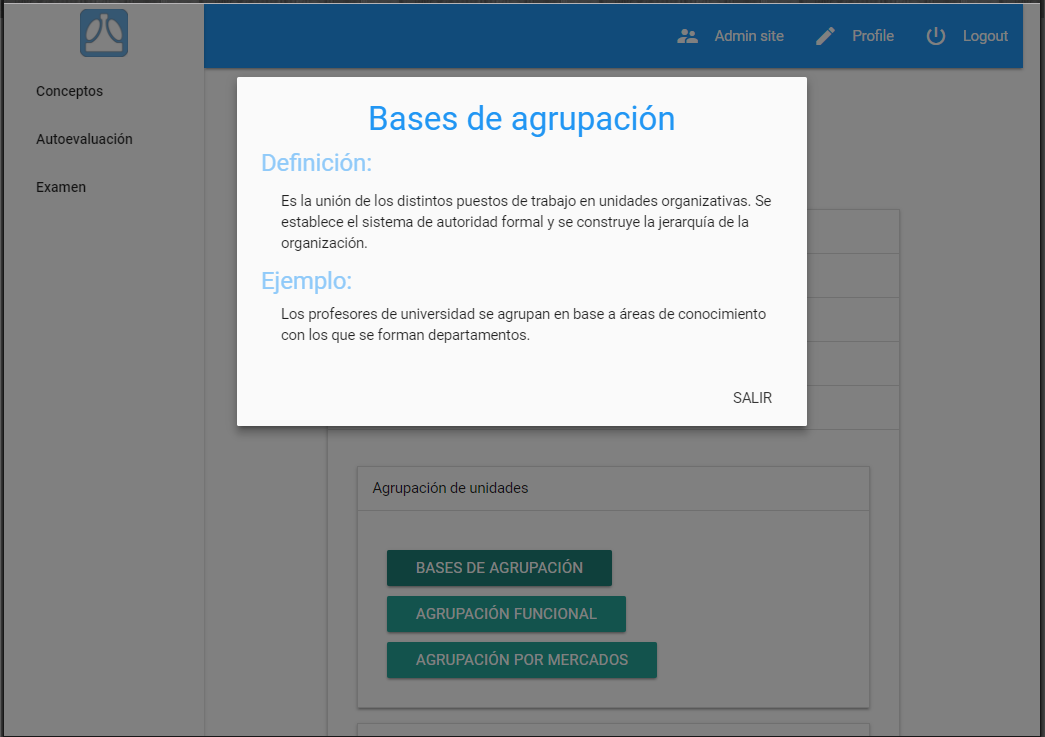
\includegraphics[width=1\textwidth]{../images/interfaz_conceptos2.png}
    \caption{Interfaz de usuario conceptos 2/2.}
    \label{fig:interfaz_conceptos2}
  \end{center}
\end{figure}


\begin{figure}[!ht]
  \begin{center}
    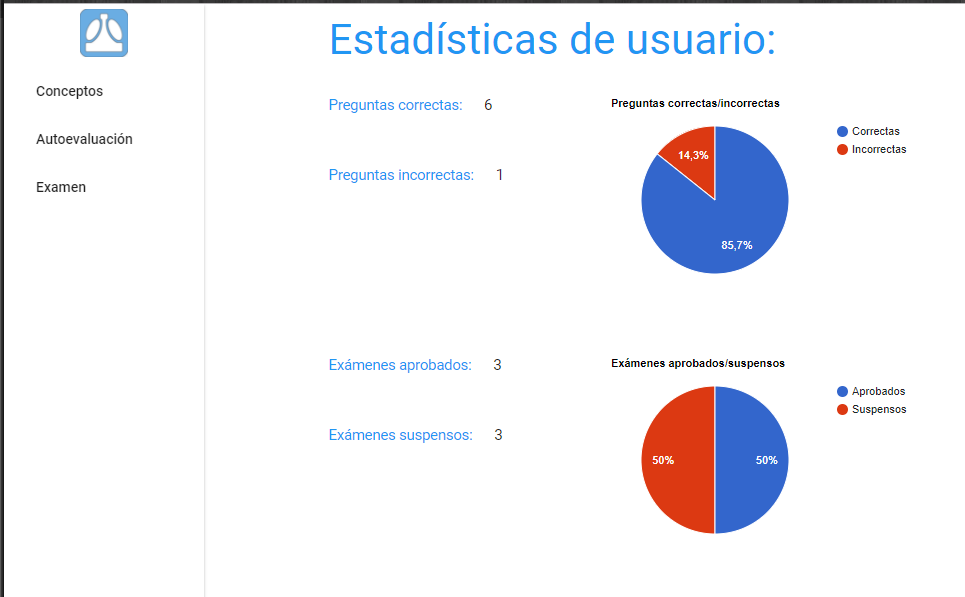
\includegraphics[width=1\textwidth]{../images/interfaz_estadisticas.png}
    \caption{Interfaz de usuario estadísticas de usuario.}
    \label{fig:interfaz_estadisticas}
  \end{center}
\end{figure}



\newpage

\section{Implementación}

Para una correcta y efectiva implementación destacaremos una vez más la importancia del proceso de análisis y diseño. Son en estas fases donde se asienta la implementación y si las anteriores se hicieron correcta y detalladamente esta fase se convierte en una mera interpretación o traducción de los análisis, diagramas y diseños anteriores. 

\bigskip
Para la fase de implementación es importante conocer las herramientas de las que podemos hacer uso. Nuestra aplicación se establece en un entorno web y ya hicimos un pequeño sondeo de las tecnologías que podíamos utilizar, ahora vamos a hablar brevemente de cómo hemos usado las herramientas y lenguajes en la implementación.

\bigskip
Vamos a distinguir entre lenguajes y herramientas usadas en el lado del cliente y lenguajes y herramientas usados en el lado del servidor:

\subsection{En el lado del servidor}
  En el lado del servidor tenemos Python como lenguaje y Django como framework.

\begin{itemize}
  \item \textbf{Django:} Framework web.
  \item \textbf{Python:} Lenguaje en el lado del servidor.
  \item \textbf{SQLite:} Sistema de gestión de base de datos.
\end{itemize}

\bigskip
Como ya explicamos unos capítulos atrás esta es nuestra elección para la parte del servidor. Una vez realizada la implementación podemos hablar de las experiencias con estas herramientas que ahora si, en mayor o menor medida, conocemos.

\bigskip
Lo primero que vamos a destacar es Django como framework web. Si bien es cierto que durante el {\grado} hemos trabajado con Django, lo hicimos dando unas ligeras pinceladas. En el desarrollo de este proyecto hemos podido comprobar la potencia de esta herramienta que abarca un amplio ámbito de componentes, desde la gestión de las rutas de nuestra aplicación pasando por la integración de los modelos y la base de datos hasta la gestión del controlador y las plantillas.

\bigskip
Con Django hemos conseguido abstraernos a un nivel un poco mayor de la gestión de la base de datos. Django trabaja con modelos, donde los desarrolladores definen sus ``entidades'' y Django se encarga de gestionarlas en la base de datos (que podemos definir en la configuración de Django) y en nuestro caso es SQLite. Separar estos modelos nos permite, por ejemplo, cambiar la base de datos en cualquier momento y haciendo las migraciones necesarias, al hacer esto los modelos definidos en Django no sufrirán ninguna modificación.

\bigskip
De manera similar diferenciar entre los modelos, vistas y plantillas nos permite realizar un cambio en cualquiera de estos sistemas sin tener que cambiar sustancialmente el otro. Esto ha sido especialmente útil en este proyecto al cambiar la conexión de los modelos a las hojas de Google Drive. En una primera prueba de conexión entre Django y Google Drive, la lectura de varias celdas se hacía algo lenta. A medida que maduraba la implementación dimos con una forma de recorrer estos datos de manera más eficiente. La gestión de los modelos y el cambio que esto supuso no interfirió con las vistas ni las plantillas ya creadas lo que facilitó esta tarea.

\bigskip
También vamos a destacar que, a nuestro parecer, la curva de aprendizaje de Django es algo complicada. Se necesita tiempo para asimilar los diferentes conceptos que trabaja y los diferentes paquetes que podemos utilizar, cosa que creemos normal en un framework de estas dimensiones. A cambio, la potencia que ofrece este framework es más que notable.




\subsection{En el lado del cliente}

\begin{itemize}
  \item \textbf{Html5:} Lenguaje de marcado para las plantillas. 
  \item \textbf{CSS3:} Lenguaje que define los estilos de las plantillas.
  \item \textbf{LESS:} Precompilador CSS.
  \item \textbf{MaterializeCss:} Framework CSS ``responsive"\footnote{Que se adapta a varias resoluciones de pantalla}
  \item \textbf{jQuery:} Biblioteca multiplataforma de JavaScript.
\end{itemize}


\bigskip
Para mostrar la información en una aplicación web podríamos decir que lo básico que necesitamos es un lenguaje de marcado (Html5) y un lenguaje con el que definir sus estilos (CSS3). En nuestra aplicación, al igual que nos servimos de paquetes y frameworks en la parte del servidor para no rehacer funcionalidades a bajo nivel, en la parte del cliente nos basaremos en estilos ya predefinidos que nos ayudarán a dar un aspecto a la aplicación. Para esto hemos elegido MaterializeCss que nos permite agrupar los tamaños y colores de los elementos de la aplicación, así como facilitarnos funcionalidades como expandir y contraer listas, mostrar u ocultar el menú lateral en resoluciones de pantalla pequeñas, mostrar ventanas modales y crear la vista de formularios. Para esta interacción y la gestión de estos eventos se hace uso de jQuery.


\bigskip
Aunque relacionado con la parte del cliente no se especificaron muchos requisitos podemos hacer referencia al RNF-3 (\ref{rnf-3}) donde nos ha sido muy útil MaterializeCss ya que los elementos usados de este framework se ajustan a los diferentes tamaños de pantalla.



\subsection{Otras herramientas}

\begin{itemize}
  \item \textbf{PyCharm:} 
  \bigskip
    En general el uso de PyCharm como entorno de programación lo podemos calificar como positivo. Destacamos la ayuda que ofrece el entorno a la sintaxis del lenguaje, que al ser nuevo nos costó un poco al inicio de la implementación, o a la gestión y uso de las bibliotecas de Django por su extensión.
    \bigskip
    Señalar algunos puntos negativos que creemos que son comunes a cualquier entorno de programación y es la sensación de no saber qué está pasando en algunos momentos al incluir paquetes externos. Esto se produce por la automatización casi total de las funciones para agregar paquetes. Como caso particular al incluir el paquete de LESS el sistema no lo reconocía, tras varios intentos desinstalando e instalando con PyCharm se decidió hacerlo manualmente desde la terminal.

  \item \textbf{Git y Github:}
  \bigskip
   Ya describimos anteriormente Git pero creemos interesante contar las conclusiones sacadas de Git y Pycharm.
  
  \bigskip
  Ya en el {\grado} hemos hecho uso de Git como herramienta de control de versiones, pero siempre desde la terminal. La sincronización de Git y Pycharm resultó útil en cuanto a la visualización de ficheros incluidos en el repositorio y los que aún quedaban  por incluir o por subir al repositorio. Pycharm los cataloga con color verde (los actualizados en el repositorio), rojos(los que no están actualizados) y grises(los que no están incluidos). De esta forma en la barra lateral del entorno puedes ver rápidamente cómo están tus ficheros en el repositorio.
  
  \bigskip
  Por otro lado, la herramienta gráfica para la gestión del repositorio no resulta intuitiva y útil, quizá por ser usuarios asiduos a Git desde la terminal, pareciendo que no controlas completamente la actualización del repositorio. En este proyecto no se ha usado Git integrado con Pycharm y la gestión se ha realizado desde la terminal.
  
  \bigskip
  \textbf{GitHub} es una plataforma donde podemos conectar nuestros repositorios de Git de forma pública o privada. Los repositorios públicos forman una comunidad con código enorme de diferentes lenguajes y plataformas y con diferentes licencias de uso. 
  
  \bigskip
  En el proyecto hemos conectado Github con nuestros dos repositorios, uno se destina al código fuente y otro para el desarrollo en LaTex de esta misma documentación. El por qué de separar estos repositorios lo desarrollaremos más adelante.

  \begin{itemize}
    \item \textbf{Código fuente: }\href{https://github.com/rogegg/iOrg2}{https://github.com/rogegg/iOrg2} 
    \item \textbf{Documentación: }\href{https://github.com/rogegg/iOrg2_docu}{https://github.com/rogegg/iOrg2_docu} 
  \end{itemize}

  \item \textbf{Heroku:}
  \bigskip
  Heroku es una plataforma como servicio de computación en la Nube que soporta distintos lenguajes de programación. Esta plataforma nos va a permitir desplegar nuestro servidor en la nube y acercarnos al entorno final de producción de la aplicación. Llegados a este punto vemos interesante explicar cómo hemos hecho el despliegue y cómo hemos subido nuestra aplicación a la plataforma, vamos a extenderlo en el próximo capítulo.

\end{itemize}